\section{Slacklining variations and categorization}\label{3_2_slacklineVariations}
Further depending on the length, tension or height a few slackline variations have originated~\cite{MillerMauser2013-sl, Kleindl2011-bl, Thomann2017-ab}. Regarding the height one can differentiate between a \textit{lowline} and a \textit{highline} (Figure \ref{fig:lowAndHighline}). The former is the category in which almost all lines match because it describes a height in which one can safely jump off the line. On a \textit{highline} this is not possible. Here you have to make safety provisions like a seperate system where the person can hook herself in this system above or under the regular line~\cite{Kleindl2011-bl}.
\begin{figure}[htb]
	\centering
	\begin{minipage}[t]{0.44\linewidth}
		\centering
		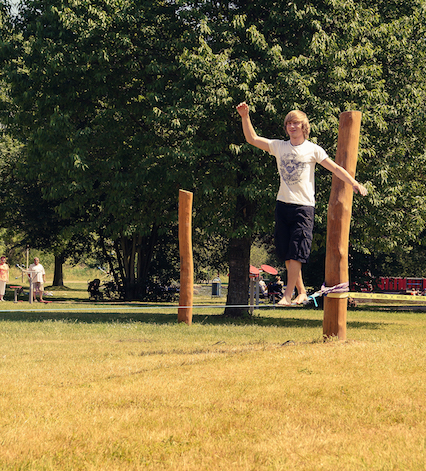
\includegraphics[width=0.94\linewidth]{Pictures/3_1_lowline}
		\subcaption{Common lowline}
		\label{fig:lowline}
	\end{minipage}
	\hfill
	\begin{minipage}[t]{0.44\linewidth}
		\centering
		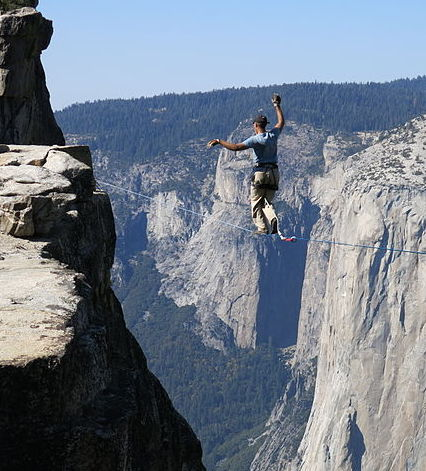
\includegraphics[width=0.94\linewidth]{Pictures/3_1_highline2}
		\subcaption{Highline between mountains~\cite{WikiSlacklining2017-lowline}}
		\label{fig:highline}
	\end{minipage}
	\caption{Low- and Highline}
	\label{fig:lowAndHighline}
\end{figure}

The following terms describe some categorization of the slackline in different application scenarios, which can differ in its scenario or blend into each other. The simple \textit{trickline} is the common slackline. It is tensed a bit loose in about the height of the knees and has a length up to 30 m. A \textit{jumpline} is stronger tensed to make jumps on the line possible. They have a length of 8 - 14 m and are a bit higher than the trickline. 

With a \textit{rodeoline} the line is actually more slacked and and has the highest amplitude. It is a relatively short line with a length of 5 - 8 m and the fixation points are in about 2 m such that if a person stands in the mid of the line it is just about above the ground and can swing on it. Slacklines beyond 30 m are called \textit{longline}. The goal here is to walk as far as possible without falling off the line. Beside these there exist also \textit{waterlines}, which is simply a slackline tensed over water and an \textit{urbanline} where manmade or urban structures are used to tense the line between.
\begin{figure}[htb]
	\centering
	\begin{minipage}[t]{0.45\linewidth}
		\centering
		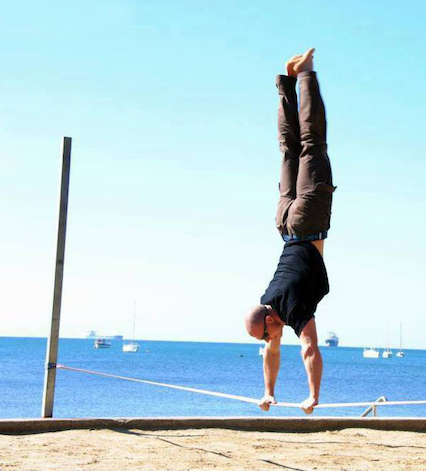
\includegraphics[width=1\linewidth]{Pictures/3_1_trickline}
		\subcaption{Handstand on a trickline~\cite{WikiSlacklining2017-trickline}}
		\label{fig:trickline}
	\end{minipage}
	\hfill
	\begin{minipage}[t]{0.45\linewidth}
		\centering
		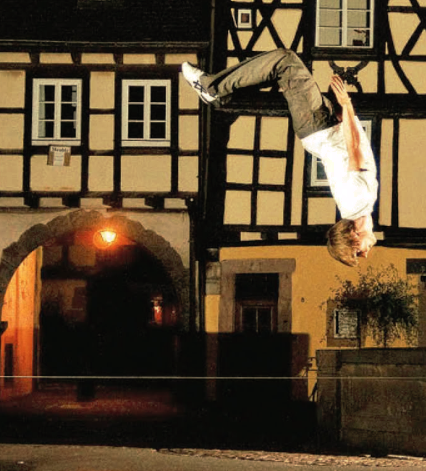
\includegraphics[width=1\linewidth]{Pictures/3_1_jumpline}
		\subcaption{Backflip on a jumpline~\cite{Kleindl2011-bl}}
		\label{fig:jumpline}
	\end{minipage}
	\hfill
	\begin{minipage}[t]{0.45\linewidth}
		\centering
		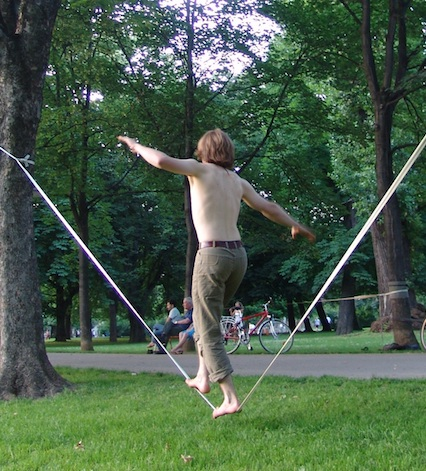
\includegraphics[width=1\linewidth]{Pictures/3_1_rodeoline}
		\subcaption{Rodeoline~\cite{WikiSlacklining2017-rodeoline}}
		\label{fig:rodeoline}
	\end{minipage}
	\hfill
	\begin{minipage}[t]{0.45\linewidth}
		\centering
		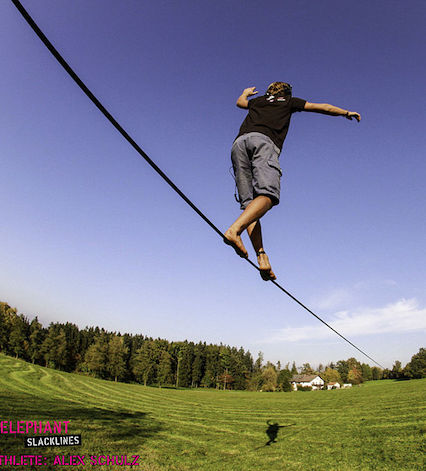
\includegraphics[width=1\linewidth]{Pictures/3_1_longline1}
		\subcaption{Longline~\cite{WikiSlacklining2017-longline}}
		\label{fig:longline}
	\end{minipage}
	\caption{Slackline variations}
	\label{fig:slacklineVariation}
\end{figure}
\clearpage
\begin{figure}[htb]
	\centering
	\begin{minipage}[t]{0.45\linewidth}
		\centering
		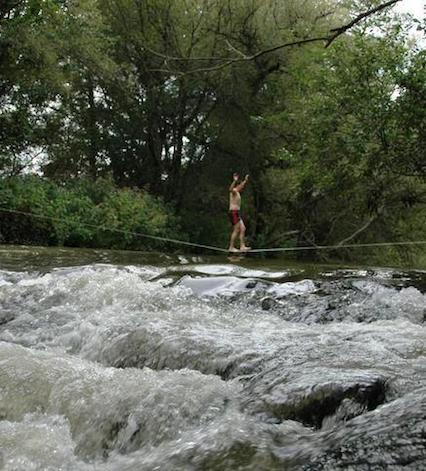
\includegraphics[width=1\linewidth]{Pictures/3_1_waterline}
		\subcaption{Waterlining over a river~\cite{WikiSlacklining2017-waterline}}
		\label{fig:waterline}
	\end{minipage}
	\hfill
	\begin{minipage}[t]{0.45\linewidth}
		\centering
		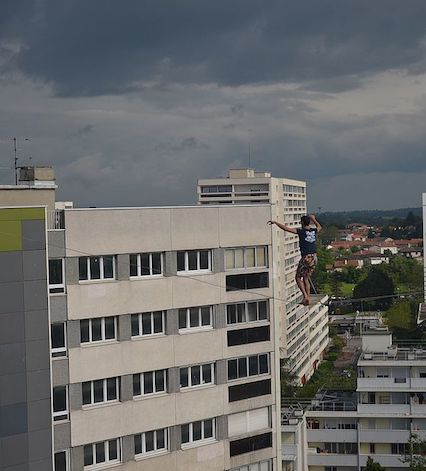
\includegraphics[width=1\linewidth]{Pictures/3_1_urbanline}
		\subcaption{Urbanlining in the city~\cite{WikiSlacklining2017-urbanline}}
		\label{fig:urbanline}
	\end{minipage}
	\caption{Categorization of slacklining}
	\label{fig:slacklineCategorization}
\end{figure}

